%\documentclass[draft]{elsarticle}
\documentclass{elsarticle}
\usepackage[margin=2.5cm]{geometry}

%%% STUFF THAT WE WANT TO INCLUDE IN THE THESIS.  THIS PART WAS NOT INCLUDED IN
%THE THESIS TEMPLATE PROVIDED BY THE DEPT. -DS.

%%%%% Uncommenting these three lines breaks the whole build ... ! -DS

%\newtheorem*{thm}{Theorem}

\usepackage{epsfig,psfrag}
\usepackage{amsmath}
\usepackage{amssymb}
\usepackage{latexsym,pifont,color,comment}
\usepackage{mathtools}
\usepackage{Logemann}
\usepackage{Integral}
\usepackage{Derivative}
\usepackage{Sum}
\usepackage{booktabs}

% command for vector notation
\renewcommand{\v}[1]{\mathbf{#1}}

\newcommand{\Tau}{\mathrm{T}}

\newcommand{\R}{\mathbb{R}}
\newcommand{\reals}{\mathbb{R}}

% left superscript macro -see
% http://www.math.leidenuniv.nl/~edix/public_html_rennes/sgahtml/typesetting_rules.html
\newcommand{\leftexp}[2]{{\vphantom{#2}}^{#1}{#2}}

\newcommand{\tens}[1]{\ensuremath{\overset{\leftrightarrow}{#1}}}
\newcommand{\mbf}[1]{\text{\mbox{\boldmath{\(#1\)}}}}
\newcommand{\inwhite}[1]{\mbox{\color{white} #1}}
\renewcommand\O{\mathcal{O}}

\newcommand{\Tm}{{\mathcal{T}}}
\newcommand{\de}{\delta}
\newcommand{\Av}{{\mathbb{A}}}
\newcommand{\xv}{{\bf x}}
\newcommand\x{{\bf x}}
\renewcommand\u{{\bf u}}
\newcommand{\nv}{{\bf n}}
\newcommand{\X}{X}
\newcommand{\Y}{Y}
\newcommand{\C}{C}
\newcommand{\D}{D}
\newcommand{\dist}{\text{\bf dist}}
\newcommand{\Bm}{{\mathcal{B}}}
\newcommand{\hmet}{\tens{h}}
\newcommand{\asdq}{{{\mathcal{A}}}_1^{\pm}\Delta{Q}}
\newcommand{\bsdq}{{{\mathcal{A}}}_2^{\pm}\Delta{Q}}
\newcommand{\apdq}{{{\mathcal{A}}}_1^{+}\Delta{Q}}
\newcommand{\bpdq}{{{\mathcal{A}}}_2^{+}\Delta{Q}}
\newcommand{\amdq}{{{\mathcal{A}}}_1^{-}\Delta{Q}}
\newcommand{\bmdq}{{{\mathcal{A}}}_2^{-}\Delta{Q}}
\newcommand{\deldot}{\vec{\nabla} \cdot}
\newcommand{\A}{\mathbb{A}}
\newcommand{\Om}{{\mathcal{O}}}
\newcommand{\pt}{{\frac{\partial}{\partial{} t}}}
\newcommand{\pk}{{\frac{\partial}{\partial{} x^k}}}
\newcommand{\Ft}{\tilde{F}}
\newcommand{\fwave}{{\mathcal{Z}}}
\newcommand{\id}{{\mathbb{I}}}

%commands for the non-dimensionalization:

\newcommand{\ft}{\tilde{f}}
\newcommand{\xt}{\tilde{x}}
\newcommand{\vt}{\tilde{v}}

\newcommand{\Et}{\tilde{E}}
\newcommand{\Bt}{\tilde{B}}

\newcommand{\phit}{\tilde{\phi}}
\newcommand{\nt}{\tilde{n}}
\newcommand{\rhot}{\tilde{\rho}}
\newcommand{\meter}{\text{m}}
\newcommand{\Volts}{\text{Volts}}
\newcommand{\farad}{\text{F}}
\newcommand{\kg}{\text{kg}}
\newcommand{\coulomb}{\text{C}}
\newcommand{\tit}{\tilde{t}}

\newcommand{\bb}[1]{{\bf #1}}

% nondimensionalized with vectors instead of scalars:
% bold - tilde - n
\newcommand{\bEt}{\tilde{\bf E}}
\newcommand{\bBt}{\tilde{\bf B}}
\newcommand\bvt{{\tilde{\bf v}}}
\newcommand\bxt{{\tilde{\bf x}}}


% electric and magnetic fields
\newcommand\E{{\bf E}}
\newcommand\B{{\bf B}}
\def\J{{\bf J}}

% Used for writing norms:
\providecommand{\norm}[1]{\lVert#1\rVert}

\newcommand{\half}{\frac{1}{2}}

% for operator split section:
\newcommand\oA{{\mathcal{A}}}
\newcommand\oB{{\mathcal{B}}}

% for Poisson equation solver in (2+2)D
% \def\v{{\bf v}}
\def\x{{\bf x}}
\def\u{{\bf u}}
\def\c{{\bf c}}
\def\En{{\mathcal{E}}}
\def\NF{{\mathcal{F}}}
\def\EL{{\mathbb{E}}}
\def\PL{{\mathbb{P}}}
\def\bmu{\mbf{\nu}}

\def\B{{\bf B}}
\def\half{\frac{1}{2}}
\def\En{{\mathcal{E}}}
\def\E{{\bf E}}
\def\J{{\bf J}}
\def\ft{\tilde{f}}
\def\tti{\tilde{t}}
\def\xt{\tilde{x}}
\def\vt{\tilde{v}}
\def\Et{\tilde{E}}
\def\rhot{\tilde{\rho}}
\def\Flux{{\mathcal{F}}}

\newcommand{\M}[1]{M_{#1}}

\usepackage{algorithm,algorithmic}
\usepackage{amsthm}
\newtheorem{theorem}{Theorem}[section]
%\theoremstyle{remark}
%\newtheorem*{rmk}{Remark}
\newtheorem{remark}{Remark}

\journal{J. Comput. Appl. Math.}

\begin{document}

\begin{frontmatter}

%\title{Asymptotic-Preserving Quadrature-Based Moment-Closure Methods
%for the Vlasov-Poisson-\\ Fokker-Planck System in the High-Field Limit}

\title{An Implicit-Explicit Discontinuous Galerkin Scheme using a Newton-Free Picard Iteration for a Thin-Film Model}

\author[author1]{Caleb Logemann}
\ead{logemann@iastate.edu}

\author[author1]{James A. Rossmanith\fnref{labc}}
\ead{rossmani@iastate.edu}

\address[author1]{Iowa State University, Department of Mathematics,
396 Carver Hall, Ames, IA 50011, USA}

%\address[author2]{Iowa State University, Department of Mathematics,
%396 Carver Hall, Ames, IA 50011, USA}



\fntext[labc]{Corresponding author}

\begin{abstract}
  This paper provides a high-order numerical scheme for solving thin-film models of the
  form \(q_t + \p{q^2 - q^3}_x = -\p{q^3 q_{xxx}}_x\).
  The second term in this equation is of nonlinear hyperbolic type, while the right-hand
  side is of nonlinear parabolic type.
  The nonlinear hyperbolic term is discretized with the standard modal discontinuous
  Galerkin method, and the nonlinear parabolic term is discretized with the local
  discontinuous Galerkin method.
  Propagation in time is done with an implicit-explicit Runge-Kutta scheme so as to
  allow for larger time steps.
  The timestep restriction for these methods is determined by the hyperbolic wavespeed
  restriction, and is not limited by the nonlinear parabolic term.
  % TODO: Describe as a linearization or state that only 1 Picard iteration is needed to converge
  A novel aspect of this method is that the resulting nonlinear algebraic equations
  are solved with a Newton-free iteration with a Picard iteration.
  The number of iterations required to converge is less than or equal to the estimated
  order of the method.
  We have demonstrated with this method up to third order convergence.
\end{abstract}

\begin{keyword}
Discontinuous Galerkin; High-Order Schemes; Implicit-Explicit; Newtwon-Free; Picard Iteration; Thin-Film Models
\end{keyword}

\end{frontmatter}

% !TEX root = main.tex

\section{Introduction}\label{sec:intro}
  In this paper we look at the model equation,
  \begin{equation}
    q_t + \p{q^2 - q^3}_x = -\p{q^3 q_{xxx}}_x \quad (x, t) \in \br{a, b} \times \br{0, T}. \label{eq:thin_film_model}
  \end{equation}
  This equation describes the motion of a thin film of liquid flowing over a
  one-dimensional domain, \(\br{a, b}\), where \(q(x, t) \ge 0\) is the height of the
  liquid.
  This fluid is acted upon by gravity, by forces on the surface, and by surface tension.
  The surface forces can have many different causes, including wind shear forces,
  thermocapillary forces, or molecular forces.
  In all cases an equivalent model can be derived.
  This model is useful in many different applications including airplane
  de-icing~\cite{article:myers2002slowly, article:myers2002flow} and industrial coating.
  Some experimental study~\cite{article:cazabat1990fingering,
  article:kataoka1997theoretical, article:ludviksson1971dynamics} has been done and
  numerical results have shown good agreement with those experiments
  in~\cite{article:bertozzi1998contact}.

  Previous numerical methods for this type of equation have focused on finite difference
  approaches.
  Bertozzi and Brenner~\cite{bertozzi1997linear} used a fully implicit centered finite
  difference scheme to explore instabilities.
  Ha et al.~\cite{article:Ha2008} explored several different finite difference schemes,
  some fully implicit and some using the Crank-Nicolson method.
  In their analysis, they considered several different methods for the hyperbolic terms
  including WENO, Godunov, and an adapted upwind method.
  All of these methods were limited to just first or second order, and they required
  solving a Newton iteration.
  Finite difference methods also lack provable stability.
  % other drawbacks to finite difference methods

  We chose to use discontinuous Galerkin methods as they allow for high order
  convergence.
  The discontinuous Galerkin methods were first introduced by Reed and
  Hill~\cite{techreport:Reed1973}, and then were formalized by Cockburn and Shu
  in a series of papers~\cite{article:Cockburn1991I, article:Cockburn1989II,
  article:Cockburn1989III, article:Cockburn1990IV, article:cockburn1998V}.
  We use the original modal discontinuous Galerkin method as well as the local
  discontinuous Galerkin method.
  The local discontinuous Galerkin method was also formulated by Cockburn and
  Shu~\cite{article:Cockburn1998LDG} to handle convection-diffusion equations with the
  discontinuous Galerkin method.
  We use the modal discontinuous Galerkin method to discretize the convection term,
  \(\p{q^2 - q^3}_x\), and
  the local discontinuous Galerkin method to discretize the diffusion term,
  \(-\p{q^3 q_{xxx}}_x\).

  The nonlinear diffusion is much stiffer, as it has an infinite wavespeed, than the
  hyperbolic convection, which only has a finite wavespeed.
  If the diffusion is handled explicitly in time, then a very strict time step
  restriction is needed to insure stability.
  Therefore the nonlinear diffusion should be solved implicitly.
  The whole system could be solved implicitly, however we chose to use an
  implicit-explicit (IMEX) Runge-Kutta scheme for propagating in time.
  These schemes were first introduced by Ascher et al.~\cite{article:ascher1997implicit}
  and have been expanded on by Kennedy and Carpenter~\cite{kennedy2003additive} and
  Pareschi and Russo~\cite{article:pareschi2000IMEX}.
  The IMEX Runge-Kutta schemes allows us not only to solve the nonlinear diffusion
  implicitly, but it also allows for the nonlinear convection to be propagated
  explicitly.
  Solving the convection explicitly fully captures the nonlinear behavior without a
  nonlinear solve.

  The diffusion still requires a nonlinear solve, but this is simpler than solving both
  convection and diffusion nonlinearly.
  We solve the nonlinear system using a Picard iteration, first introduced by {\'E}mile
  Picard and then formalized by Lindel{\"o}f~\cite{lindelof1894application}.
  We find that very minimal number of iterations is required for the iteration to
  converge.
  In fact we find one iteration allows for high order convergence of smooth solutions,
  and that one iteration provides good results for travelling shock solutions.
  With these methods we have demonstrated up to third order accuracy with a manufactured
  solution example.
  We also demonstrate the nonlinear traveling wave behavior through several numerical
  examples introduced by Bertozzi~\cite{article:Bertozzi1999}.
  These examples demonstrate that the steady state traveling wave may not be unique.
  They also show a double shock structure with an undercompressive shock.
% !TEX root = main.tex

\section{The Thin-Film Model}\label{sec:equations}
  In this model we consider a thin film of liquid on a flat surface with a free
  interface.
  This liquid is driven by gravity, shear and normal forces on the surface, and surface
  tension (see Figure~\ref{fig:thin_film}).
  We begin by considering the two dimensional incompressible Navier-Stokes equations,
  which have the form,
  \begin{align}
    u_x + w_z &= 0, \label{eq:incompressibility}\\
    \rho\p{u_t + u u_x + w u_z} &= -p_x + \mu \Delta u - \phi_x, \label{eq:con_mom1}\\
    \rho\p{w_t + u w_x + w w_z} &= -p_z + \mu \Delta w - \phi_z, \label{eq:con_mom2}
  \end{align}
  where \(\rho \) is the density, \(u\) is the horizontal velocity, \(w\) is the
  vertical velocity, \(p\) is the pressure, and \(\phi \) is the force of gravity.
  Equation~\eqref{eq:incompressibility} is the incompressibility condition and also
  represents conservation of mass.
  Equations~\eqref{eq:con_mom1} and~\eqref{eq:con_mom2} represent the conservation of
  momentum in the \(x\) and \(z\) directions respectively.
  We take a no penetration and no slip boundary condition at the lower boundary and the
  kinematic boundary condition at the upper boundary.
  These boundary conditions can be expressed as follows,
  \begin{align}
    w &= 0, \quad u = 0, &\text{at } z = 0, \\
    w &= h_t + u h_x, &\text{at } z = h,
  \end{align}
  where \(h\) is the height of the liquid.
  We can also describe the stress tensor, \(\v{T}\), at the free surface, \(z = h\),
  as
  \begin{align*}
    \v{T} \cdot \v{n} &= \p{-\kappa \sigma + \Pi_0}\v{n}
      + \p{\pd{\sigma}{s} + \tau_0}\v{t}, &\text{at } z = h,
  \end{align*}
  where \(\kappa \) is the mean curvature, \(\sigma \) is the surface tension, and
  \(\Pi_0 \) and \(\tau_0 \) are the normal and tangential components of the forcing
  respectively.

  \begin{figure}
    \centering
    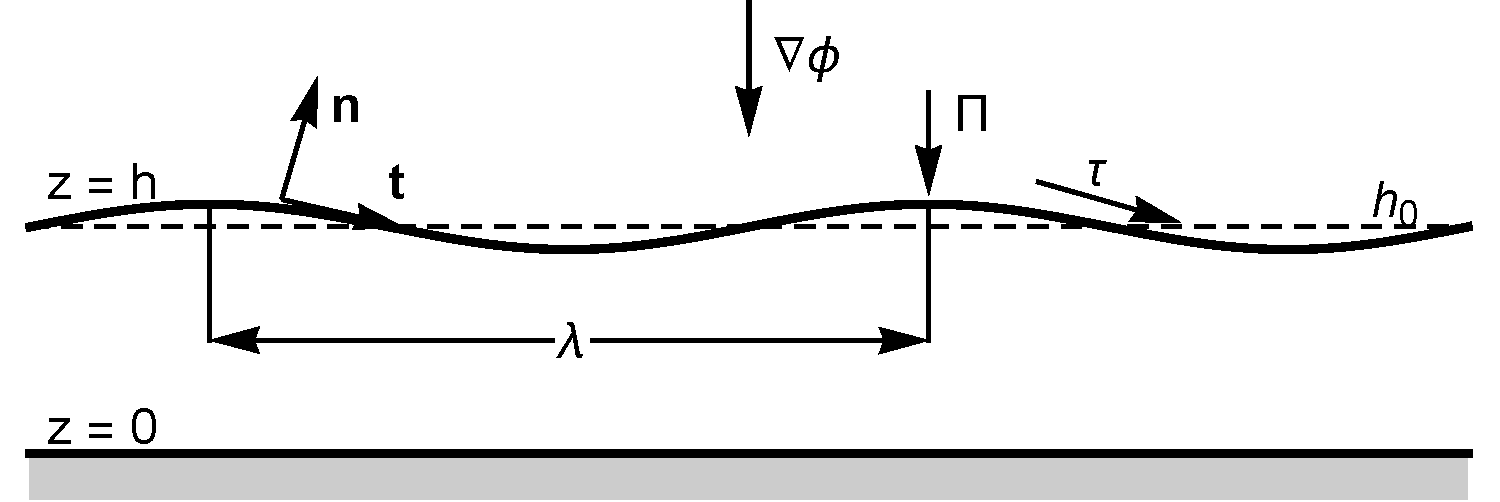
\includegraphics[scale=0.45]{figures/ThinFilm.pdf}
    \caption{A diagram of the Thin-Film Model}\label{fig:thin_film}
  \end{figure}

\subsection{Derivation}
  These equations completely describe the fluid, but we are now going to make a
  lubrication approximation, through a scaling argument similar to that given by Oron
  et al.~\cite{oron1997long}.
  For the lubrication approximation we are going to assume that the average height of
  the liquid, \(h_0\), is much smaller then the characteristic wavelength of the liquid,
  \(\lambda \).
  We will denote the ratio of these two lengths as \(\varepsilon \), that is
  \begin{equation}
    \varepsilon = \frac{h_0}{\lambda} \ll 1.
  \end{equation}
  Now we nondimensionalize the rest of the variables with respect to this ratio.
  We denote the nondimensional variables as the uppercase variables.
  As we stated earlier the characteristic height is \(h_0\) and the characteristic
  length is \(\lambda = h_0/\varepsilon \), so the nondimensional length variables are
  \begin{equation}
    Z = \frac{z}{h_0}, \quad X = \frac{\varepsilon x}{h_0}, \quad H = \frac{h}{h_0}.
  \end{equation}
  Let \(U_0\) be the characteristic horizontal velocity, then
  \begin{equation}
    \quad U = \frac{u}{U_0}, \quad W = \frac{w}{\varepsilon U_0},
  \end{equation}
  where the nondimensional vertical velocity, \(W\), follows from the continuity
  equation.
  It follows that time will be scaled by \(\lambda/U_0\), so nondimensional time is
  \begin{equation}
    T = \frac{\varepsilon U_0 t}{h_0}.
  \end{equation}
  Finally we assume that the flow is locally parallel or equivalently
  \(p_x \sim \mu u_{zz}\).
  This gives us the proper scaling for the pressure, gravity, and surface stresses,
  \begin{equation}
    P = \frac{\varepsilon h_0}{\mu U_0} p, \quad
    \Phi = \frac{\varepsilon h_0}{\mu U_0}\phi, \quad
    \Pi = \frac{\varepsilon h_0}{\mu U_0}\Pi_0, \quad
    \tau = \frac{h_0}{\mu U_0}\tau_0.
  \end{equation}
  Lastly we can nondimensionalize the surface tension as
  \begin{equation}
    \Sigma = \frac{\varepsilon \sigma}{\mu U_0}.
  \end{equation}
  Substituting these nondimensional variables into the original equations gives
  \begin{align}
    U_X + W_Z &= 0, \\
    \frac{\varepsilon U_0 \rho h_0}{\mu}\p{U_T + UU_X + WU_Z} &=
    -P_X + \p{\varepsilon^2 U_{XX} + U_{ZZ}} - \Phi_X, \\
    \varepsilon^3 \frac{\rho U_0 h_0}{\mu}\p{W_T + UW_X + WW_Z} &=
    -P_Z + \varepsilon^2\p{\varepsilon^2 W_{XX} + W_{ZZ}} - \Phi_Z,
  \end{align}
  at \(Z = 0\)
  \begin{gather}
    W = 0, \quad U = 0,
  \end{gather}
  and at \(Z = H\)
  \begin{gather}
    W = H_T + U H_x, \\
    -P - \Pi + \frac{2 \varepsilon^2}{1 + \varepsilon^2 H_X^2} \Big(\p{\varepsilon^2 H_X^2 U_X + W_Z} \nonumber \\
    - H_X \p{U_Z + \varepsilon^2 W_X}\Big) = \frac{\varepsilon^2 H_{XX}}{\p{1 + \varepsilon^2 H_X^2}^{3/2}} \Sigma, \\
    2 \varepsilon^2 H_X \p{W_Z - U_X} + \p{1 - \varepsilon^2 H_X^2} \p{U_Z + \varepsilon^2 W_X} \nonumber \\
    = \Sigma_X \p{1 + \varepsilon^2 H_X^2}^{1/2} + \tau \p{1 + \varepsilon^2 H_X^2}.
  \end{gather}

  We can now let \(\varepsilon \to 0\) which results in
  \begin{align}
    U_X + W_Z &= 0, \label{eq:nd_continuity}\\
    P_X + \Phi_X &= U_{ZZ}, \label{eq:nd_con_mom1} \\
    P_Z + \Phi_Z &= 0, \label{eq:nd_con_mom2}
  \end{align}
  at \(Z = 0\),
  \begin{gather}
    W = 0, \quad U = 0, \\
  \end{gather}
  and at \(Z = H\)
  \begin{align}
    W &= H_T + U H_x,  \\
    -P - \Pi &= \bar{\Sigma} H_{XX}, \\
    U_Z &= \Sigma_X + \tau.
  \end{align}
  Note that we assume that the surface tension is large, so that
  \(\bar{\Sigma} = \varepsilon^2 \Sigma = O(1)\).
  This is important in order to keep surface tension effects in the final equation.

  Lastly we integrate these equations over \(Z\) and apply the boundary conditions,
  in order to integrate out all of the variables except the free surface height, \(H\).
  Integrating equation~\eqref{eq:nd_continuity} gives
  \begin{equation}
    H_T + \pda{\dintt{0}{H}{U}{Z}}{X} = 0,
  \end{equation}
  and integrating equation~\eqref{eq:nd_con_mom1} twice gives
  \begin{equation}
    U = \p{\tau + \Sigma_X}Z + \p{P_X + \Phi_X}\p{\frac{1}{2} Z^2 - HZ},
  \end{equation}
  and finally integrating equation~\eqref{eq:nd_con_mom2} gives
  \begin{equation}
    P + \Phi = \eval{\Phi}{Z=H} - \Pi - \bar{\Sigma} H_{XX}.
  \end{equation}
  Substituting all of these equations together results in
  \begin{equation}
    H_T + \p{\frac{1}{2}\p{\tau + \Sigma_X}H^2 - \frac{1}{3}\p{\eval{\Phi}{Z=H} - \Pi}_X H^3}_X = - \p{\bar{\Sigma} H^3 H_{XXX}}_X.
  \end{equation}
  Setting all the constants to 1 and using the variable \(q\) instead gives us our
  original model equation~\eqref{eq:thin_film_model}.

\subsection{Hyperbolic Convection Dynamics}
  Consider the thin-film model with only the hyperbolic convection term, that is
  \begin{equation}
    q_t + \p{q^2 - q^3}_x = 0.
  \end{equation}
  Equations of the type \(q_t + f\p{q}_x = 0\) are known as conservation laws, where
  \(f\) is called the flux function.
  The dynamics of this equation are determined by the flux function.
  In the system case, the conservation law is called hyperbolic at \(q\) if \(f'(q)\)
  is diagonalizable with real eigenvalues.
  In the scalar case, this reduces to having a real valued flux function, so this term
  is indeed hyperbolic.
  We also need to consider if our flux function is convex or nonconvex.
  It is known that \(f\) is nonconvex if
  \(f''(q) = 0\) for some \(q\).
  In our case \(f''(q) = 2 - 6q\), so \(f''(q) = 0\) at \(q = \frac{1}{3}\).
  We can also see in Figure~\ref{fig:flux_function} that there is an inflection
  point at \(q = \frac{1}{3}\).
  Nonconvex flux functions can exhibit more complex behavior than convex flux
  functions.
  Nonconvex flux functions can involve compound waves including rarefaction-shocks.
  See Leveque~\cite{leveque2002finite} for more details.

  \begin{figure}
    \centering
    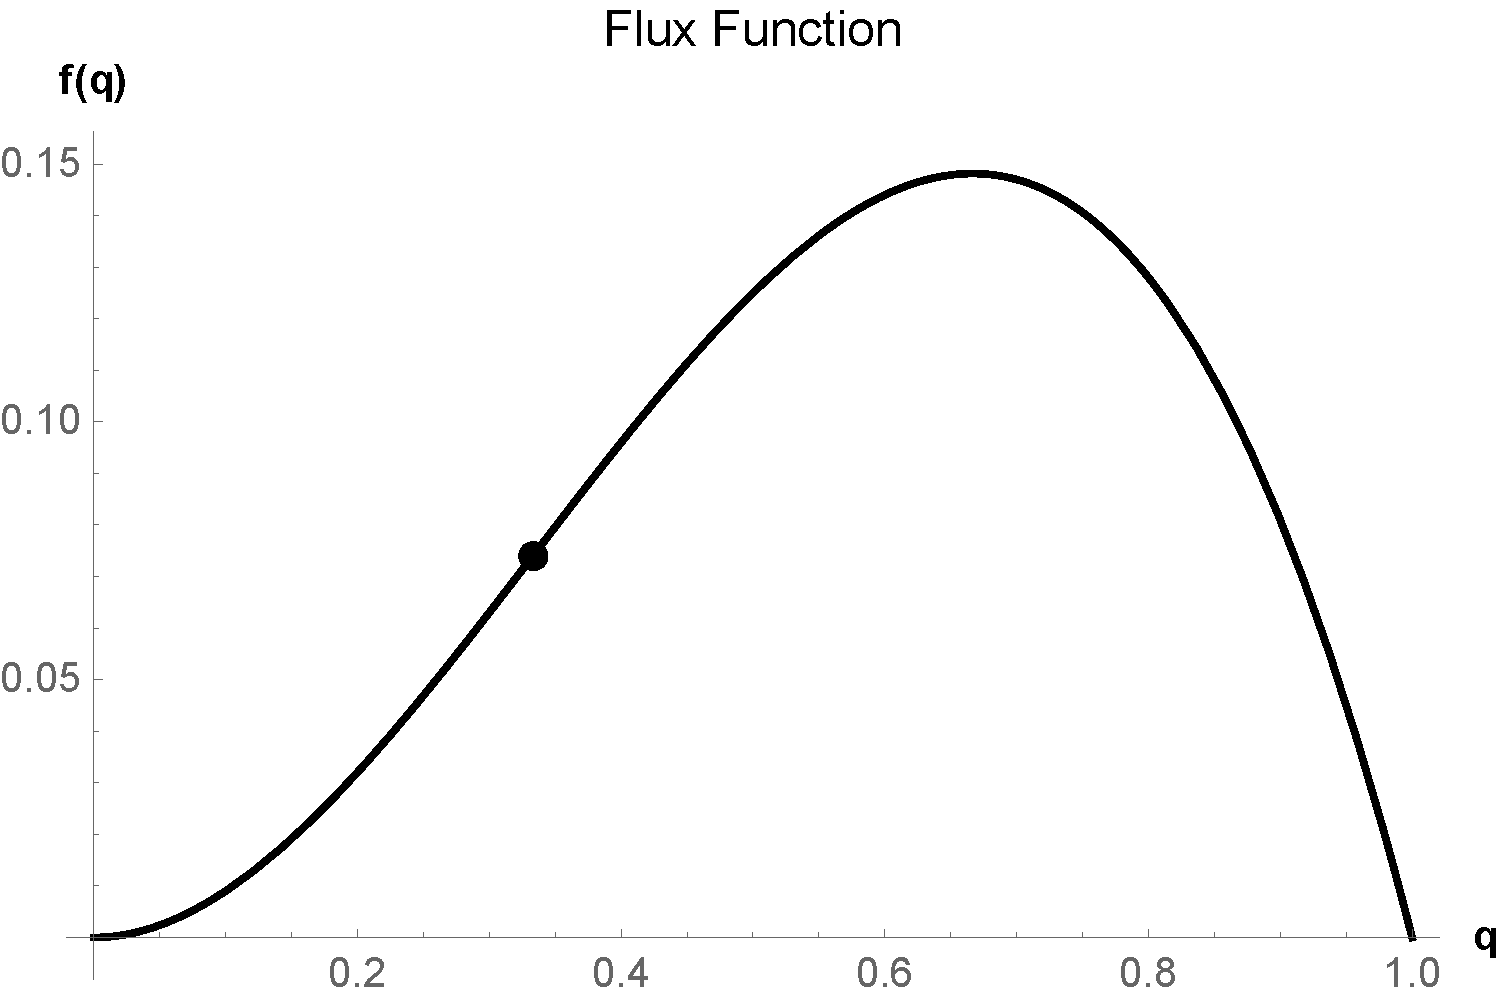
\includegraphics[scale=0.3]{figures/FluxFunctionNonconvex.pdf}
    \caption{Plot of flux function, \(f(q) = q^2 - q^3\).}\label{fig:flux_function}
  \end{figure}

  Another interesting feature of hyperbolic equations is that they have a finite
  wavespeed.
  The wavespeed of the conservation law is determined by \(f'(q)\).
  In our case, \(f'(q) = 2q - 3q^2\), so the wavespeed can be as large as
  \(\frac{1}{3}\).
  Having a finite wavespeed can be very useful for numerical methods, as this limits
  the speed of propagation of information.
  Each point in the domain has a finite radius of influence for each future time.

\subsection{Parabolic Dynamics}
  Now consider the thin-film model with only the parabolic term, that is
  \begin{equation}
    q_t = -\p{q^3 q_{xxx}}_x.
  \end{equation}
  Using the product rule of differentiation this is equivalent to
  \begin{equation}
    q_t = -\p{3q^2 q_x} q_{xxx} - q^3 q_{xxxx}.
  \end{equation}
  The dynamics of the third and fourth derivative terms can be analyzed with the
  Fourier transform.

  Consider, \(q_t = -q_{xxx}\), and take the Fourier transform of both sides, which
  results in
  \begin{equation}
    \mathcal{F}\p{q}_t = -i \xi^3 \mathcal{F}(q).
  \end{equation}
  Solving this ordinary differential equation (ODE) gives
  \begin{equation}
    \mathcal{F}\p{q} = e^{-i \xi^3 t}.
  \end{equation}
  We know that this type of solution has a dispersive dynamics.

  Similarly consider, \(q_t = -q_{xxxx}\), and take the Fourier transform of both sides.
  This gives the following ordinary differential equation
  \begin{equation}
    \mathcal{F}\p{q}_t = -\xi^4 \mathcal{F}(q).
  \end{equation}
  The solution to this ODE is
  \begin{equation}
    \mathcal{F}\p{q} = e^{-\xi^4 t}.
  \end{equation}
  This is a function that decays rapidly in time, and the higher the wavenumber,
  \(\xi \), the faster the diffusion.

  Therefore we expect this parabolic term to exhibit dispersive and diffusive dynamics.
  The dynamics are also nonlinearly coupled together making the behavior even more
  difficult to predict.
  The one thing that is clear is that the overall model is very stiff.
  The vast time scale difference between the finite wavespeed of the hyperbolic
  convection and the rapid decay of the nonlinear diffusion, make this model very stiff.
  Our numerical method must be able to handle this stiffness in a way that is not too
  computationally intensive.
% !TEX root = main.tex

\section{Numerical Methods}\label{sec:numerical}

  \subsection{Implicit-Explicit Runge-Kutta Scheme}\label{ssec:imex}
    The thin-film model we are trying to solve is a very stiff equation due to the
    high order derivatives.
    In order to take reasonable timesteps despite this stiffness we use
    implicit-explicit (IMEX) Runge-Kutta schemes to propagate our solution through time.
    The IMEX Runge-Kutta scheme propagates time for ordinary differential
    equations or systems of equations of the form
    \begin{equation}
      q_t = F(t, q) + G(t, q),
    \end{equation}
    where \(F\) is solely handled explicitly, but \(G\) needs to be solved implicitly.
    A single step of the Runge-Kutta IMEX scheme is computed as follows,
    \begin{align}
      q^{n+1} &= q^n + \Delta t \sum{i = 1}{s}{b_i' F(t_i, u_i)} + \Delta t \sum{i=1}{s}{b_i G(t_i, u_i)} \\
      u_i &= q^n + \Delta t \sum{j = 1}{i-1}{a_{ij}' F(t_j, u_j)} + \Delta t \sum{j=1}{i}{a_{ij} G(t_j, u_j)} \\
      t_i &= t^n + c_i \Delta t
    \end{align}
    where the coefficients \(a_{ij}\), \(b_i\), \(c_i\), \(a_{ij}'\), \(b_i'\), and
    \(c_i'\) are set in the double Butcher tableau
    \begin{center}
      \begin{tabular}{r|l}
        \(c'\) & \(a'\) \\
        \midrule
          & \(\p{b'}^T\)
      \end{tabular}\hspace{0.5cm}
      \begin{tabular}{r|l}
        \(c\) & \(a\) \\
        \midrule
          & \(b^T\)
      \end{tabular}.
    \end{center}

    Specifically we used the IMEX schemes first introduced by Pareschi and
    Russo~\cite{article:pareschi2000IMEX, article:pareschi2005IMEX}.
    These schemes are strong stability preserving (SSP) in the sense of Gottlieb et
    al.~\cite{gottlieb2001strong} and they are designed for stiff systems.
    The double Butcher tableaus are shown below for the one stage, L-stable, 1st order
    method:
    \begin{center}
      \begin{tabular}{r|l}
        0 & 0 \\
        \midrule
          & 1
      \end{tabular}\hspace{0.5cm}
      \begin{tabular}{r|l}
        1 & 1 \\
        \midrule
          & 1
      \end{tabular},
    \end{center}
    the three stage, 2nd order method:
    \begin{center}
      \begin{tabular}{r|lll}
        0 & 0 & 0 & 0 \\
        0 & 0 & 0 & 0 \\
        1 & 0 & 1 & 0 \\
        \midrule
          & 0 & \(\frac{1}{2}\) & \(\frac{1}{2}\) \\
      \end{tabular}\hspace{0.5cm}
      \begin{tabular}{r|lll}
        \(\frac{1}{2}\) & \(\frac{1}{2}\) & 0 & 0 \\
        0 & \(-\frac{1}{2}\) & \(\frac{1}{2}\) & 0 \\
        1 & 0 & \(\frac{1}{2}\) & \(\frac{1}{2}\) \\
        \midrule
          & 0 & \(\frac{1}{2}\) & \(\frac{1}{2}\) \\
      \end{tabular},
    \end{center}
    and the four stage, L-stable, third order method:
    \begin{center}
      \begin{tabular}{r|llll}
        0 & 0 & 0 & 0 & 0 \\
        0 & 0 & 0 & 0 & 0 \\
        1 & 0 & 1 & 0 & 0 \\
        \(\frac{1}{2}\) & 0 & \(\frac{1}{4}\) & \(\frac{1}{4}\) & 0 \\
        \midrule
          & 0 & \(\frac{1}{6}\) & \(\frac{1}{6}\) & \(\frac{2}{3}\) \\
      \end{tabular} \hspace{0.5cm}
      \begin{tabular}{r|llll}
        \(\alpha \) & \(\alpha \) & 0 & 0 & 0 \\
        0 & \(-\alpha \) & \(\alpha \) & 0 & 0 \\
        1 & \(0\) & \(1 - \alpha \) & \(\alpha \) & 0 \\
        \(\frac{1}{2}\) & \(\beta \) & \(\eta \) & \(\zeta \) & \(\alpha \) \\
        \midrule
          & 0 & \(\frac{1}{6}\) & \(\frac{1}{6}\) & \(\frac{2}{3}\) \\
      \end{tabular}, \\
    \end{center}
    where
    \begin{center}
      \begin{align*}
        \alpha &= 0.24169426078821, \\
        \beta &= 0.06042356519705, \\
        \eta &= 0.1291528696059, \\
        \zeta &= \frac{1}{2} - \beta - \eta - \alpha.
      \end{align*}
    \end{center}

    For our thin-film model \(F\) and \(G\) will be the spatial discretizations of
    the hyperbolic convection and parabolic terms respectively, that is
    \begin{align}
      F(t, q) &= -\p{q^2 - q^3}_x \\
      G(t, q) &= -\p{q^3 q_{xxx}}_x.
    \end{align}
    Since \(G\) is the stiffest part of our model, we would like to handle this term
    implicitly so that our time step is less restricted.
    Also handling \(F\) explicitly allows us to capture the nonlinear
    behavior without a nonlinear solve.

  \subsection{Space Discretization}
    We chose to use the discontinuous Galerkin Method to discretize our equation in
    space.
    First let \(\set{x_{j+1/2}}_0^N\) partition the domain, \(\br{a, b}\), and denote
    each interval as \(I_j = \br{x_{j-1/2}, x_{j+1/2}}\) with
    \(\Delta x_j = x_{j+1/2} - x_{j-1/2}\).
    The discontinuous Galerkin solution then exists in the following finite dimensional
    space,
    \begin{equation}
      V_h^k = \set{v \in L^1\p{\br{a, b}}: \eval{v}{I_j} \in P^k(I_j), j = 1, \ldots, N},
    \end{equation}
    where \(P^k(I_j)\) denotes the set of polynomials of degree k or less on \(I_j\).

  \subsubsection{Modal Discontinuous Galerkin for Hyperbolic Convection}\label{ssec:dg}
    First we consider the continuous operator \(F(t, q) = -\p{q^2 - q^3}_x\).
    Note that \(F: \br{0, T} \times C^1(a, b) \to C^0(a, b)\), and we would like to
    form an approximation, \(F_h\) to this continuous operator, such that
    \(F_h: \br{0, T} \times V_h^k \to V_h^k\).
    In order to do this, consider the weak formulation of the continuous operator,
    \(F\).
    The weak form requires finding \(F(t, q) \in C^0(a, b)\) such that
    \begin{equation}
      \dintt{a}{b}{F(t, q) v(x)}{x} = -\dintt{a}{b}{\p{q^2 - q^3}_x v(x)}{x}
    \end{equation}
    for all smooth functions, \(v \in C^{\infty}(a, b)\).
    The discontinuous Galerkin approximation is formed by replacing these function
    spaces with the DG space, \(V_h^k\).
    This gives that the weak formulation of the approximation \(F_h\) is to find
    \(F_h(t, q_h) \in V_h^k\) such that
    \begin{equation}
      \dintt{a}{b}{F_h(t, q_h) v_h(x)}{x} = -\dintt{a}{b}{\p{q_h^2 - q_h^3}_x v_h(x)}{x}
    \end{equation}
    for all \(v_h \in V_h^k\).
    Using integration by parts this is equivalent to
    finding \(F_h(t, q_h) \in V_h^k\) such that
    \begin{align}
      \dintt{I_j}{}{F_h(t, q_h)v_h(x)}{x} &= \dintt{I_j}{}{\p{q_h^2 - q_h^3} v_h'(x)}{x} \\
      &- \hat{f}\p{q_h}_{j+1/2} v_h(x_{j+1/2}) + \hat{f}\p{q_h}_{j-1/2} v_h(x_{j-1/2}) \nonumber
    \end{align}
    for \(j = 1, \ldots, N\) and for all \(v_h \in V_h^k\).
    Since \(q_h\) is discontinuous at the cell interfaces \(x_{j\pm 1/2}\), some
    numerical flux \(\hat{f}\) must be chosen.

    We chose to use the Local Lax-Friedrich's numerical flux, that is
    \begin{equation}
      \hat{f}(q_l, q_r) = \frac{1}{2} \p{f(q_l) + f(q_r) - \lambda_{\text{max}} \p{q_r - q_l}}
    \end{equation}
    where \(f\) is the flux function, \(q_l\) and \(q_r\) and the left and right
    states at the interface, and \(\lambda_{\text{max}}\) is the locally maximum wavespeed,
    that is
    \begin{equation}
      \lambda_{\text{max}} = \max[q \in \br{\nu, \mu}]{f'(q)},
    \end{equation}
    where \(\nu = \min{q_l, q_r}\) and \(\mu = \max{q_l, q_r}\).
    In our case \(f(q) = q^2 - q^3\).
    At the interface \(x_{j+1/2}\) we have \(q_l = q_h^-(x_{j+1/2})\) and
    \(q_r = q_h^+(x_{j+1/2})\).

    % \begin{equation}
    %   \hat{f}\p{q_h}_{j+1/2} = \frac{1}{2} \p{\p{\p{\p{q_h^+(x_{j+1/2})}^2 - \p{q_h^+(x_{j+1/2})}^3} + \p{\p{q_h^-(x_{j+1/2})}^2 - \p{q_h^-(x_{j+1/2})}^3}}
    %   - \lambda_{\max} \p{q_h^+(x_{j+1/2}) - q_h^-(x_{j+1/2})}}
    % \end{equation}
    % where
    % \begin{equation}
    %   \lambda_{\max} = \max[q \in \br{}]{2q - 3q^2}
    % \end{equation}

  \subsubsection{Local Discontinuous Galerkin Scheme for Parabolic Term}\label{ssec:ldg}
    Next we look at the continuous operator \(G(t, q) = -\p{q^3 q_{xxx}}_x\).
    In discretizing this operator we follow the local discontinuous Galerkin (LDG) method
    first introduced by Cockburn and Shu~\cite{article:Cockburn1998LDG} for
    convection-diffusion systems.
    We first introduce three auxilliary variables, \(r, s, u\), and rewrite the equation
    as the following system,
    \begin{align}
      r &= q_x, \\
      s &= r_x, \\
      u &= s_x, \\
      G(t, q) &= -\p{q^3 u}_x.
    \end{align}
    The weak form of this system is solved by finding functions \(r, s, u, G\) such that
    \begin{align}
      \dintt{a}{b}{r(x) w(x)}{x} &= \dintt{a}{b}{q_x(x) w(x)}{x}, \\
      \dintt{a}{b}{s(x) y(x)}{x} &= \dintt{a}{b}{r_x(x) y(x)}{x}, \\
      \dintt{a}{b}{u(x) z(x)}{x} &= \dintt{a}{b}{s_x(x) z(x)}{x}, \\
      \dintt{a}{b}{G(t, q) v(x)}{x} &= -\dintt{a}{b}{\p{q^3(x) u(x)}_x v(x)}{x},
    \end{align}
    for all smooth functions \(w, y, z, v \in C^{\infty}(a, b)\).
    The LDG method arrives from applying the standard DG method to each of these
    equations.
    That is we replace the continuous function spaces with the
    discontinuous finite dimensional DG space, \(V_h^k\).
    The approximate operator \(G_h\) becomes the process of finding
    \(r_h, s_h, u_h, G_h(t, q_h) \in V_h\) such that for all test functions
    \(v_h, w_h, y_h, z_h \in V_h\) the following equations are
    satisfied
    \begin{align}
      \dintt{a}{b}{r_h w_h}{x} &= \dintt{a}{b}{\p{q_h}_x w_h}{x}, \\
      \dintt{a}{b}{s_h y_h}{x} &= \dintt{a}{b}{\p{r_h}_x y_h}{x}, \\
      \dintt{a}{b}{u_h z_h}{x} &= \dintt{a}{b}{\p{s_h}_x z_h}{x}, \\
      \dintt{a}{b}{G_h(t, q_h) v_h}{x} &= -\dintt{a}{b}{\p{q_h^3 u_h}_x v_h}{x},
    \end{align}
    given \(t\) and \(q_h \in V_h^k\).
    This is equivalent to the following equations for all \(j\), if we use integration
    by parts,
    \begin{align}
      \dintt{I_j}{}{r_h w_h}{x} &= \p{\p{\hat{q}_h w^-_h}_{j+1/2}
      - \p{\hat{q}_h w^+_h}_{j-1/2}} - \dintt{I_j}{}{q_h \p{w_h}_x}{x}, \\
      \dintt{I_j}{}{s_h y_h}{x} &= \p{\p{\hat{r}_h y^-_h}_{j+1/2}
      - \p{\hat{r}_h y^+_h}_{j-1/2}} - \dintt{I_j}{}{r_h \p{y_h}_x}{x}, \\
      \dintt{I_j}{}{u_h z_h}{x} &= \p{\p{\hat{s}_h z^-_h}_{j+1/2}
      - \p{\hat{s}_h z^+_h}_{j-1/2}} - \dintt{I_j}{}{s_h \p{z_h}_x}{x}, \\
      \dintt{I_j}{}{G_h(t, q_h) v_h}{x} &= -\p{\p{\widehat{q^3 u}_h v^-_h}_{j+1/2}
      - \p{\widehat{q^3 u}_h v^+_h}_{j-1/2}} + \dintt{I_j}{}{q_h^3 u_h \p{v_h}_x}{x},
    \end{align}
    where \(\hat{q}, \hat{r}, \hat{s}, \widehat{q^3 u}\) are suitably chosen numerical fluxes.
    A common choice of numerical fluxes are the so-called alternating fluxes, shown below
    \begin{align}
      \hat{q}_h &= q^-_h, \\
      \hat{r}_h &= r^+_h, \\
      \hat{s}_h &= s^-_h, \\
      \widehat{q^3 u}_h &= \p{q^3 u}^+_h.
    \end{align}
    These numerical fluxes are one-sided fluxes that alternate sides for each
    derivative.
    They are chosen to make this method stable, and they also allow for the auxilliary
    variables to be locally solved in terms of \(q_h\), hence where the local
    discontinuous Galerkin method gets its name.

  \subsection{Nonlinear Solver}
    Using these discretizations in the Runge-Kutta IMEX scheme, requires solving the
    nonlinear system,
    \begin{equation}
      u_i - \Delta t a_{ii} G_h(t_i, u_i) = q^n
      + \Delta t \sum{j = 1}{i-1}{a_{ij}' F_h(t_j, u_j)}
      + \Delta t \sum{j=1}{i-1}{a_{ij} G_h(t_j, u_j)},
    \end{equation}
    for \(u_i\).
    The standard approach to solving this system would be to use a Newton iteration,
    however that would require the Jacobian of the operator \(I - \Delta t a_{ii} G_h\),
    which would be relatively intractable.
    Therefore we chose to linearize this operator and use a Picard iteration instead,
    which does not require the Jacobian.

    Suppose we are trying to solve the nonlinear equation \(L(u) = b\), where
    \(L'(v, u)\) is the nonlinear operator linearized about \(v\) acting on \(u\).
    The Picard iteration for solving this nonlinear equation starts with some initial
    guess \(u_0\).
    The next solution is found by solving the following linear problem,
    \begin{equation}
      L'(u_i, u_{i+1}) = b.
    \end{equation}
    In other words the next iteration is found by solving the problem linearized about
    the the previous iteration.

    We linearize the operator \(G_h(t, q_h)\) by first linearizing \(G(t, q)\).
    The continuous operator linearized about \(v\) is given by
    \begin{equation}
      G'(v, t, q) = - \p{v^3 q_{xxx}}_x.
    \end{equation}
    The linearized discrete operator is now just the LDG method applied to this
    linearized continuous operator.

    We find that the Picard iteration approach provides good results with relatively few
    iterations.
    In fact in Section~\ref{sec:results} we show that we can achieve first, second, and
    third order accuracy with only one iteration, with an initial guess that is the
    solution from the previous stage of the IMEX Runge-Kutta scheme.
    If we are solving the nonlinear system for the first stage, then the initial guess
    is the solution from the previous timestep instead of the previous stage.
    This approach is more tractable than a Newton iteration and it converges
    quickly to the nonlinear solution.

    These methods were implemented in a python code called
    \textsc{PyDoGPack}~\cite{pydogpack} developed by the authors.
    \textsc{PyDogPack} uses the packages \textsc{NumPy}~\cite{numpy} and
    \textsc{SciPy}~\cite{scipy} extensively.
    In particular they are used to solve linear systems of equations and to integrate
    numerically.
    All of the examples and tests shown in Section~\ref{sec:results} were done using
    this code.
    % Key parts of the code are shown in Appendix~\ref{app:code}.

% Chapter 4 from the standard thesis template
%   that contains an adv. example table and figure.
 %\addtocontents{toc}{\protect\newpage}
\chapter{Results}

\section{One Dimensional Results}
\subsection{}
% 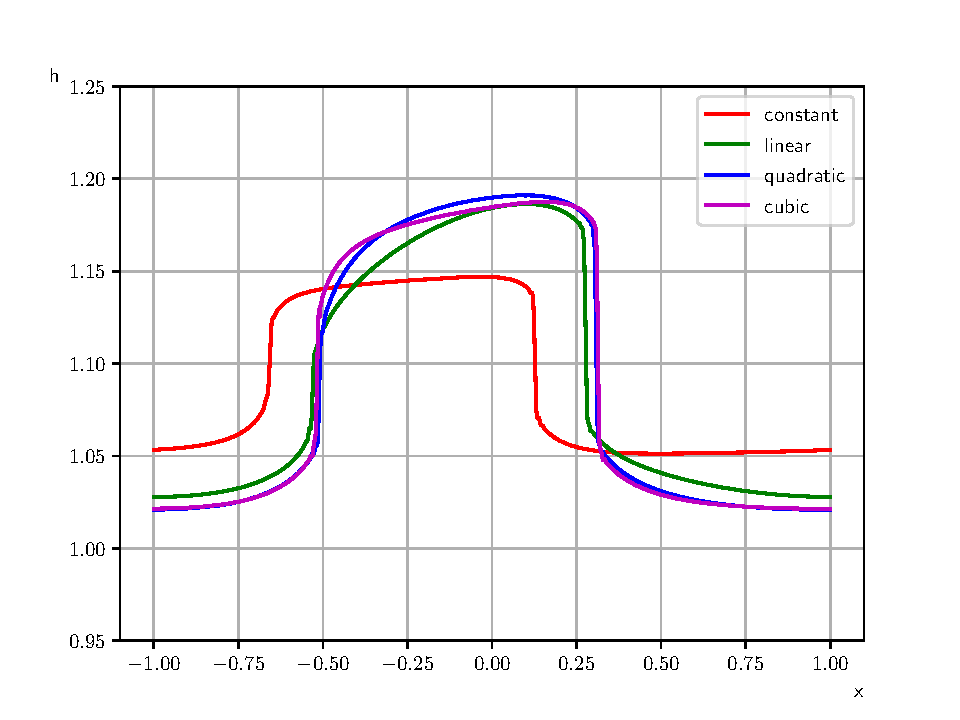
\includegraphics[scale=0.29]{Figures/height_torillhon.pdf}
% 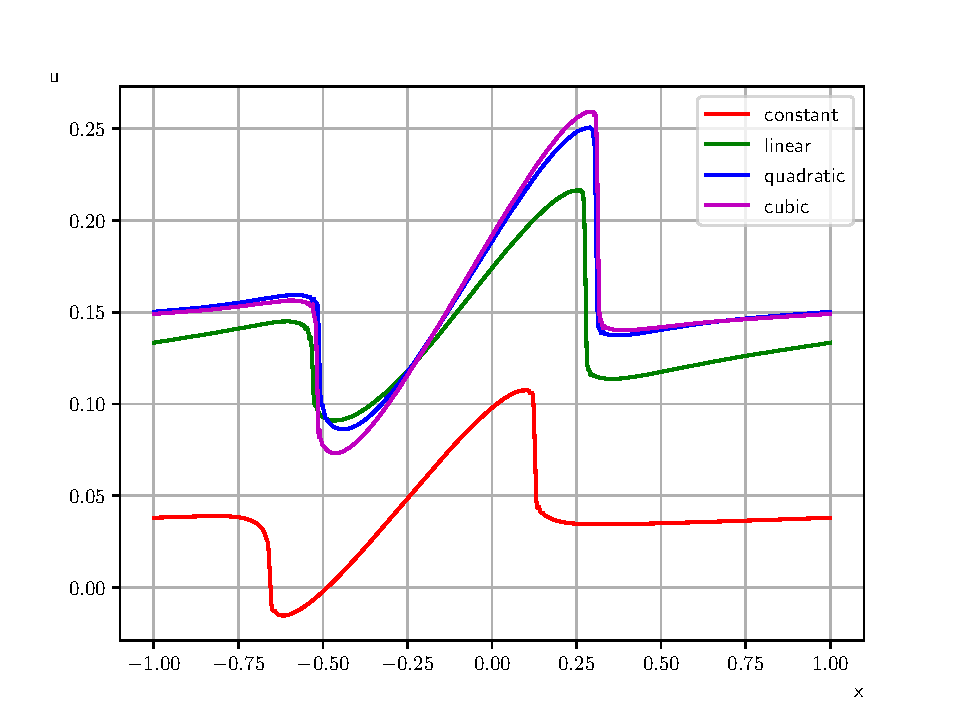
\includegraphics[scale=0.29]{Figures/mean_velocity_torrilhon.pdf}
% 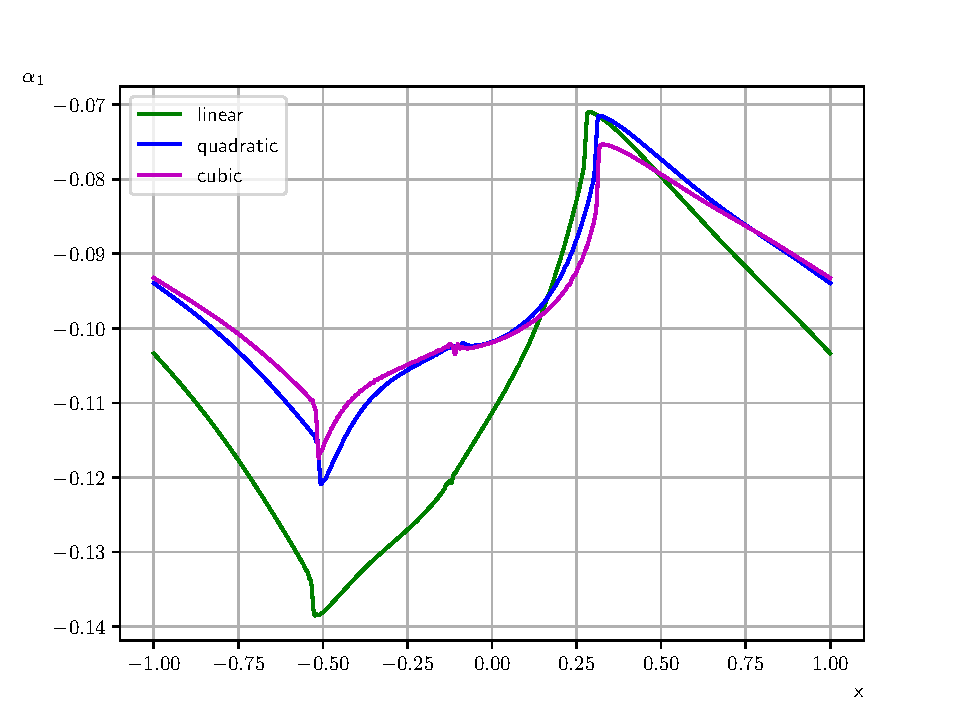
\includegraphics[scale=0.29]{Figures/alpha_1_torrilhon.pdf}
% 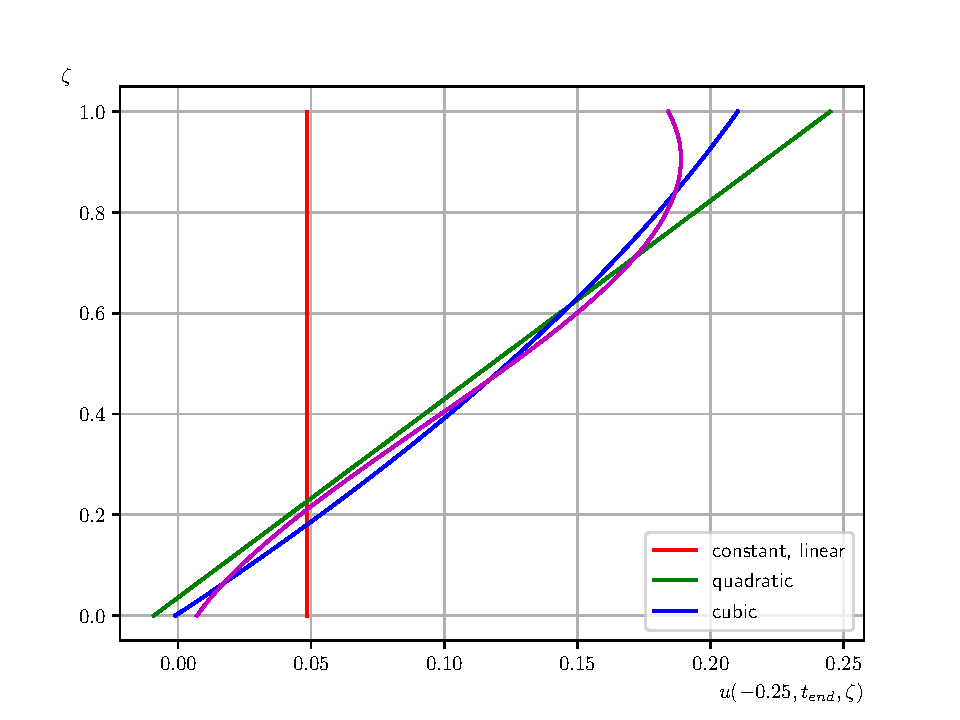
\includegraphics[scale=0.29]{Figures/velocity_profile_-025_torrilhon.pdf}
% 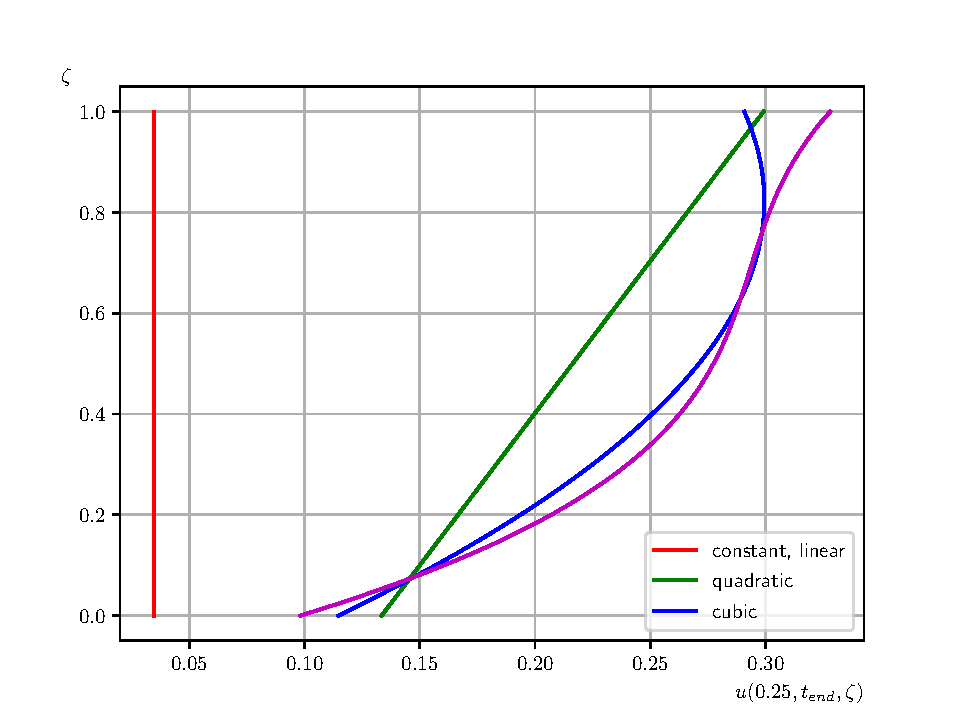
\includegraphics[scale=0.3]{Figures/velocity_profile_025_torrilhon.pdf}

% 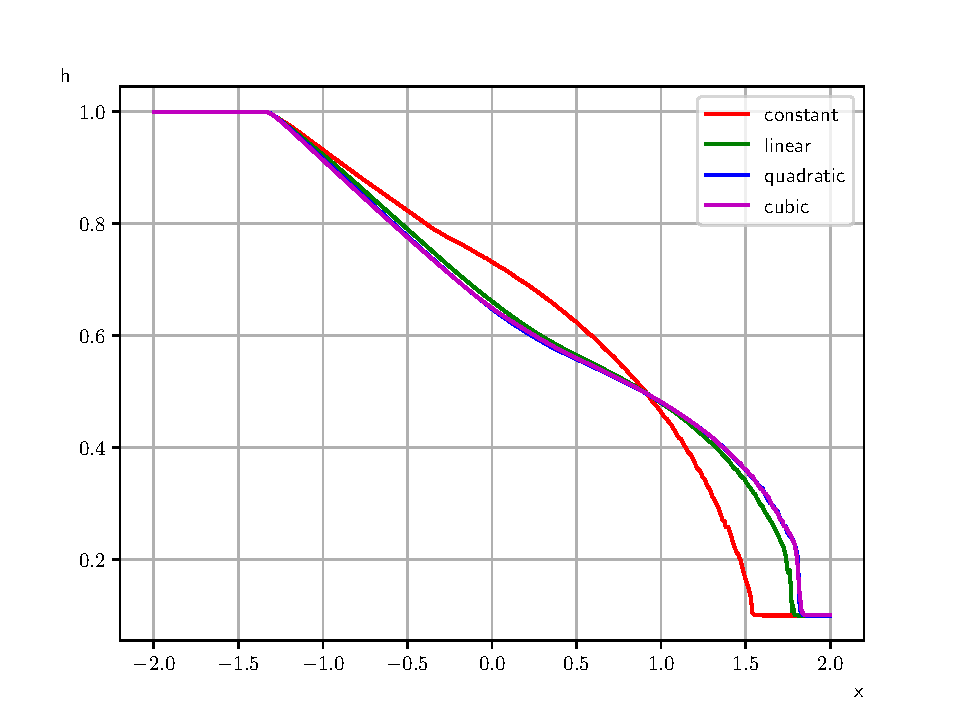
\includegraphics[scale=0.29]{Figures/height_dam.pdf}
% 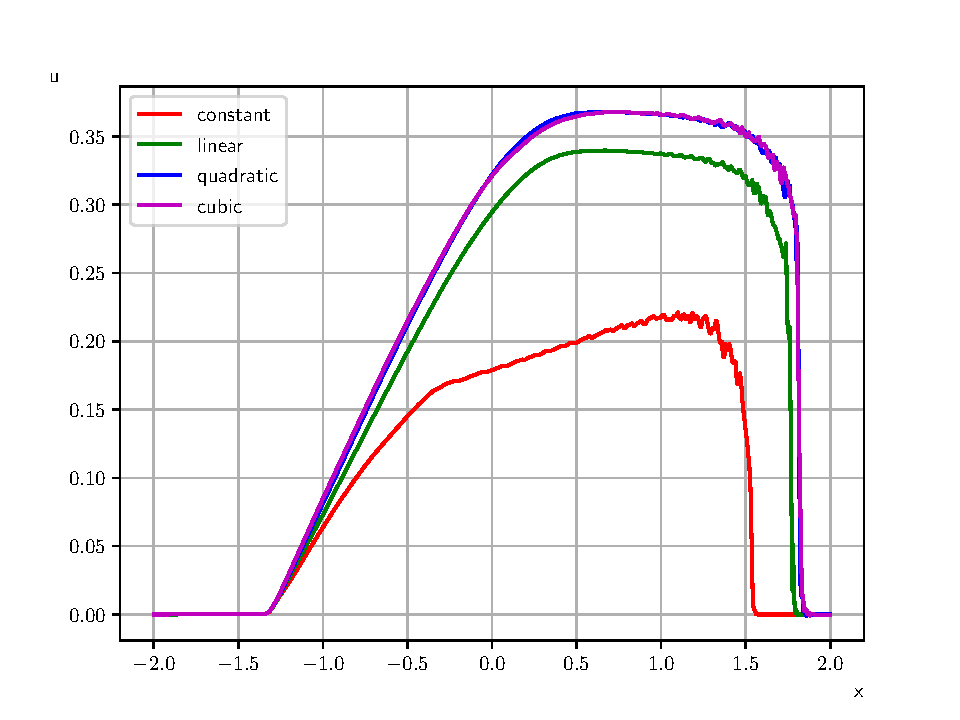
\includegraphics[scale=0.29]{Figures/mean_velocity_dam.pdf}
% 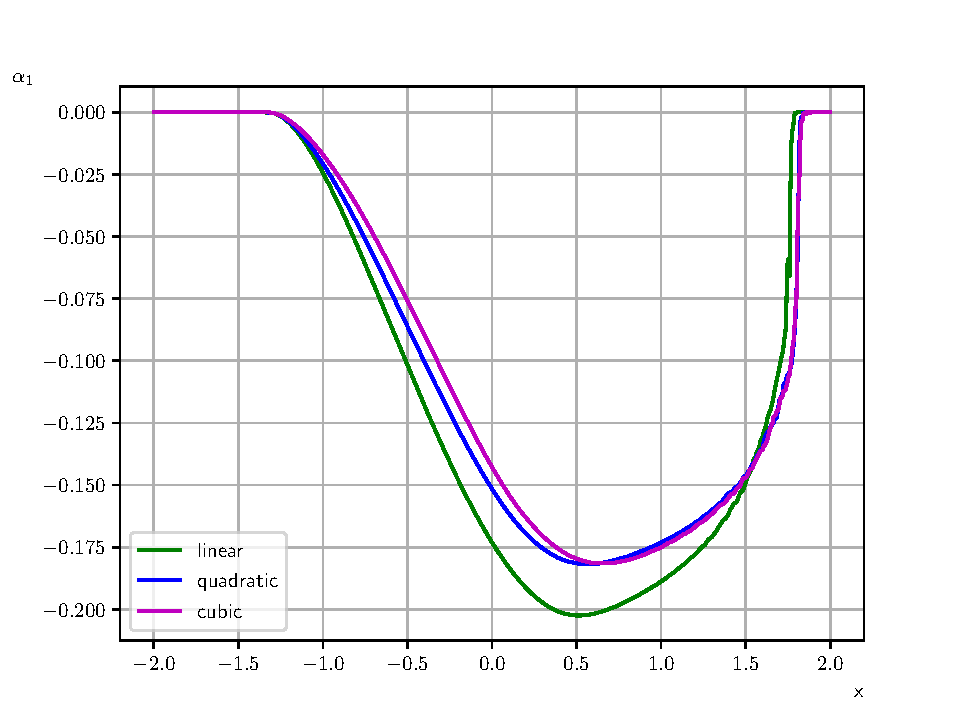
\includegraphics[scale=0.29]{Figures/alpha_1_dam.pdf}
% 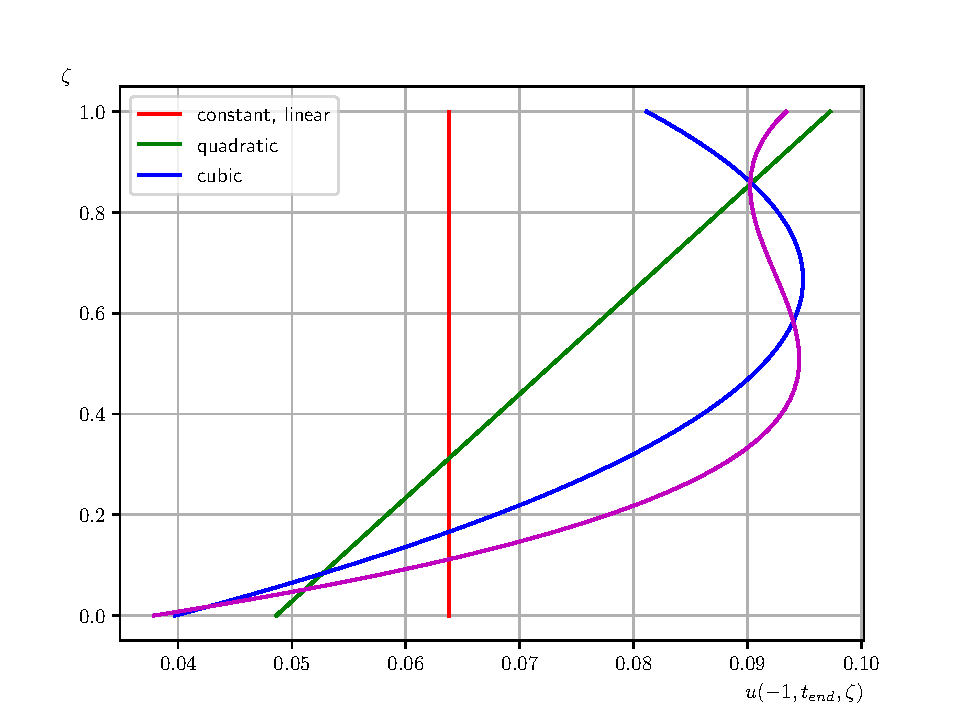
\includegraphics[scale=0.29]{Figures/velocity_profile_-1_dam.pdf}
\subsection{Manufactured Solution}
  I also ran a manufactured solution example to verify the order of convergence of the
  method.
  \begin{gather}
    q_i(x, t) = 0.1 \sin{2 \pi \p{x - t - 0.1 i}}
  \end{gather}
  
  \begin{table}
    \small
    \begin{tabular}{r*{10}l}
      \toprule
            & \multicolumn{2}{c}{1st Order} & \multicolumn{2}{c}{2nd Order} & \multicolumn{2}{c}{3rd Order} & \multicolumn{2}{c}{4th Order} & \multicolumn{2}{c}{5th Order} \\
      \midrule
      \(n\) & \multicolumn{1}{c}{error} & order & \multicolumn{1}{c}{error} & order & \multicolumn{1}{c}{error} & order& \multicolumn{1}{c}{error} & order & \multicolumn{1}{c}{error} & order \\
      \midrule
      20    & \( 0.226 \) & ---  & \( 8.57 \times 10^{-3} \) & ---   & \( 1.67 \times 10^{-4} \) & ---  & \( 3.17 \times 10^{-6}  \) & ---  & \( 7.61 \times 10^{-8}  \) & 0.00  \\
      40    & \( 0.117 \) & 0.96 & \( 2.17 \times 10^{-3} \) & 1.98  & \( 2.07 \times 10^{-5} \) & 3.02 & \( 1.98 \times 10^{-7}  \) & 4.00 & \( 2.38 \times 10^{-9}  \) & 5.00  \\
      80    & \( 0.058 \) & 1.00 & \( 5.40 \times 10^{-4} \) & 2.01  & \( 2.57 \times 10^{-6} \) & 3.01 & \( 1.24 \times 10^{-8}  \) & 4.00 & \( 7.71 \times 10^{-11} \) & 4.95  \\
      160   & \( 0.028 \) & 1.06 & \( 1.35 \times 10^{-4} \) & 2.00  & \( 3.21 \times 10^{-7} \) & 3.00 & \( 7.76 \times 10^{-10} \) & 4.00 & \( 4.04 \times 10^{-11} \) & 0.93  \\
      320   & \( 0.014 \) & 0.99 & \( 3.37 \times 10^{-5} \) & 2.00  & \( 4.01 \times 10^{-8} \) & 3.00 & \( 4.85 \times 10^{-11} \) & 4.00 & \( 8.09 \times 10^{-11} \) & -1.00 \\
      \bottomrule
    \end{tabular}
    \caption{Convergence Table for standard shallow water equations or shallow water moment equations with zero moments.}\label{tab:convergence_1d_0m}
  \end{table}
  \begin{table}
    \small
    \begin{tabular}{r*{10}l}
      \toprule
            & \multicolumn{2}{c}{1st Order} & \multicolumn{2}{c}{2nd Order} & \multicolumn{2}{c}{3rd Order} & \multicolumn{2}{c}{4th Order} & \multicolumn{2}{c}{5th Order} \\
      \midrule
      \(n\) & \multicolumn{1}{c}{error} & order & \multicolumn{1}{c}{error} & order & \multicolumn{1}{c}{error} & order & \multicolumn{1}{c}{error} & order & \multicolumn{1}{c}{error} & order\\
      \midrule
      20    & \( 2.53 \times 10^{-1} \) & ---  & \( 9.97 \times 10^{-3} \) & ---  & \( 1.71 \times 10^{-3} \) & ---  & \( 1.14 \times 10^{-4} \) & ---  & \( 2.68 \times 10^{ -5} \) & ---  \\
      40    & \( 1.30 \times 10^{-1} \) & 0.96 & \( 2.52 \times 10^{-3} \) & 1.98 & \( 3.85 \times 10^{-4} \) & 2.15 & \( 1.74 \times 10^{-5} \) & 2.72 & \( 8.01 \times 10^{ -7} \) & 5.06 \\
      80    & \( 6.47 \times 10^{-2} \) & 1.00 & \( 6.28 \times 10^{-4} \) & 2.00 & \( 6.13 \times 10^{-5} \) & 2.65 & \( 7.50 \times 10^{-7} \) & 4.53 & \( 1.53 \times 10^{ -8} \) & 5.71 \\
      160   & \( 3.13 \times 10^{-2} \) & 1.05 & \( 1.57 \times 10^{-4} \) & 2.00 & \( 9.09 \times 10^{-6} \) & 2.75 & \( 1.25 \times 10^{-7} \) & 2.59 & \( 4.04 \times 10^{-10} \) & 5.25 \\
      320   & \( 1.58 \times 10^{-2} \) & 0.99 & \( 3.92 \times 10^{-5} \) & 2.00 & \( 1.73 \times 10^{-6} \) & 2.39 & \( 8.79 \times 10^{-9} \) & 3.83 & \( 8.40 \times 10^{-11} \) & 2.27 \\
      \bottomrule
    \end{tabular}
    \caption{Convergence table for shallow water moment equations with one moment.}\label{tab:convergence_1d_1m}
  \end{table}
  \begin{table}
    \small
    \centering
    \begin{tabular}{r*{10}l}
      \toprule
            & \multicolumn{2}{c}{1st Order} & \multicolumn{2}{c}{2nd Order} & \multicolumn{2}{c}{3rd Order} & \multicolumn{2}{c}{4th Order} & \multicolumn{2}{c}{5th Order}\\
      \midrule
      \(n\) & \multicolumn{1}{c}{error} & order & \multicolumn{1}{c}{error} & order & \multicolumn{1}{c}{error} & order & \multicolumn{1}{c}{error} & order & \multicolumn{1}{c}{error} & order\\
      \midrule
      20    & \( 2.78 \times 10^{-1} \) & ---  & \( 1.14 \times 10^{-2} \) & ---  & \( 5.35 \times 10^{-3} \) & ---  & \( 3.69 \times 10^{ -4} \) & ---  & \( 5.19 \times 10^{ -5} \) & ---  \\
      40    & \( 1.42 \times 10^{-1} \) & 0.96 & \( 2.88 \times 10^{-3} \) & 1.98 & \( 6.47 \times 10^{-4} \) & 3.05 & \( 2.46 \times 10^{ -5} \) & 3.91 & \( 1.12 \times 10^{ -6} \) & 5.53 \\
      80    & \( 7.12 \times 10^{-2} \) & 1.00 & \( 7.19 \times 10^{-4} \) & 2.00 & \( 7.83 \times 10^{-5} \) & 3.04 & \( 1.40 \times 10^{ -6} \) & 4.13 & \( 1.93 \times 10^{ -8} \) & 5.86 \\
      160   & \( 3.45 \times 10^{-2} \) & 1.04 & \( 1.80 \times 10^{-4} \) & 2.00 & \( 1.27 \times 10^{-5} \) & 2.63 & \( 1.14 \times 10^{ -7} \) & 3.62 & \( 5.86 \times 10^{-10} \) & 5.04 \\
      320   & \( 1.74 \times 10^{-2} \) & 0.99 & \( 4.49 \times 10^{-5} \) & 2.00 & \( 2.55 \times 10^{-6} \) & 2.32 & \( 1.09 \times 10^{ -8} \) & 3.39 & \( 8.79 \times 10^{-11} \) & 2.74 \\
      \bottomrule
    \end{tabular}
    \caption{Convergence table for shallow water moments equations with two moments}\label{tab:convergence_1d_2m}
  \end{table}
  \begin{table}
    \small
    \centering
    \begin{tabular}{r*{10}l}
      \toprule
            & \multicolumn{2}{c}{1st Order} & \multicolumn{2}{c}{2nd Order} & \multicolumn{2}{c}{3rd Order} & \multicolumn{2}{c}{4th Order} & \multicolumn{2}{c}{5th Order} \\
      \midrule
      \(n\) & \multicolumn{1}{c}{error} & order & \multicolumn{1}{c}{error} & order & \multicolumn{1}{c}{error} & order & \multicolumn{1}{c}{error} & order & \multicolumn{1}{c}{error} & order \\
      \midrule
      20    & \( 3.02 \times 10^{-1} \) & ---  & \( 1.30 \times 10^{-2} \) & ---  & \( 7.02 \times 10^{-3} \) & ---  & \( 3.17 \times 10^{ -4} \) & ---  & \( 5.57 \times 10^{ -5} \) & ---  \\
      40    & \( 1.56 \times 10^{-1} \) & 0.96 & \( 3.28 \times 10^{-3} \) & 1.99 & \( 6.99 \times 10^{-4} \) & 3.33 & \( 2.38 \times 10^{ -5} \) & 3.73 & \( 1.10 \times 10^{ -6} \) & 5.66 \\
      80    & \( 7.81 \times 10^{-2} \) & 0.99 & \( 8.19 \times 10^{-4} \) & 2.00 & \( 1.18 \times 10^{-4} \) & 2.56 & \( 2.51 \times 10^{ -6} \) & 3.25 & \( 2.64 \times 10^{ -8} \) & 5.38 \\
      160   & \( 3.80 \times 10^{-2} \) & 1.04 & \( 2.05 \times 10^{-4} \) & 2.00 & \( 2.55 \times 10^{-5} \) & 2.22 & \( 3.17 \times 10^{ -7} \) & 2.99 & \( 1.37 \times 10^{ -9} \) & 4.27 \\
      320   & \( 1.92 \times 10^{-2} \) & 0.99 & \( 5.12 \times 10^{-5} \) & 2.00 & \( 5.11 \times 10^{-6} \) & 2.32 & \( 4.68 \times 10^{ -8} \) & 2.76 & \( 1.17 \times 10^{-10} \) & 3.55 \\
      \bottomrule
    \end{tabular}
    \caption{Convergence table for shallow water moment equations with three moments or a cubic velocity profile}\label{tab:convergence_1d_3m}
  \end{table}

\section{Two Dimensional Cartesian Results}
  \begin{table}
    \small
    \centering
    \begin{tabular}{r*{10}l}
      \toprule
            & \multicolumn{2}{c}{1st Order} & \multicolumn{2}{c}{2nd Order} & \multicolumn{2}{c}{3rd Order} & \multicolumn{2}{c}{4th Order} & \multicolumn{2}{c}{5th Order} \\
      \midrule
      \(n\) & \multicolumn{1}{c}{error} & order & \multicolumn{1}{c}{error} & order & \multicolumn{1}{c}{error} & order & \multicolumn{1}{c}{error} & order & \multicolumn{1}{c}{error} & order \\
      \midrule
      5     & \( 9.26 \times 10^{-1} \) & ---  & \( 9.42 \times 10^{-2} \) & ---  & \( 1.24 \times 10^{-2} \) & ---  & \( 2.25 \times 10^{-3} \) & ---  & \( 4.62 \times 10^{-4} \) & ---  \\
      10    & \( 5.02 \times 10^{-1} \) & 0.88 & \( 2.12 \times 10^{-2} \) & 2.16 & \( 2.77 \times 10^{-3} \) & 2.17 & \( 2.79 \times 10^{-4} \) & 3.02 & \( 4.12 \times 10^{-5} \) & 3.49 \\
      20    & \( 2.79 \times 10^{-1} \) & 0.85 & \( 5.09 \times 10^{-3} \) & 2.06 & \( 7.16 \times 10^{-4} \) & 1.95 & \( 3.43 \times 10^{-5} \) & 3.02 & \( 2.40 \times 10^{-6} \) & 4.10 \\
      40    & \( 1.43 \times 10^{-1} \) & 0.96 & \( 1.26 \times 10^{-3} \) & 2.02 & \( 1.60 \times 10^{-4} \) & 2.16 & \( 3.08 \times 10^{-6} \) & 3.48 & \( 1.23 \times 10^{-7} \) & 4.28 \\
      80    & \( 7.36 \times 10^{-2} \) & 0.96 & \( 3.13 \times 10^{-4} \) & 2.00 & \( 3.37 \times 10^{-5} \) & 2.25 & \( 2.76 \times 10^{-7} \) & 3.48 & \( 6.09 \times 10^{-9} \) & 4.34 \\
      \bottomrule
    \end{tabular}
    \caption{Convergence table for standard shallow water equations or shallow water moment equations with zero moments}\label{tab:convergence_2dr_0m}
  \end{table}

  \begin{table}
    \small
    \centering
    \begin{tabular}{r*{10}l}
      \toprule
            & \multicolumn{2}{c}{1st Order} & \multicolumn{2}{c}{2nd Order} & \multicolumn{2}{c}{3rd Order} & \multicolumn{2}{c}{4th Order} & \multicolumn{2}{c}{5th Order} \\
      \midrule
      \(n\) & \multicolumn{1}{c}{error} & order & \multicolumn{1}{c}{error} & order & \multicolumn{1}{c}{error} & order & \multicolumn{1}{c}{error} & order & \multicolumn{1}{c}{error} & order \\
      \midrule
      5     & \( 1.20 \)                 & ---  & \( 1.16 \times 10^{-1 } \) & ---  & \( 2.07 \times 10^{-2 } \) & ---  & \( 8.11 \times 10^{-3} \) & ---  & \( 1.52 \times 10^{-3} \) & ---  \\
      10    & \( 6.69 \times 10^{-1 } \) & 0.84 & \( 2.46 \times 10^{-2 } \) & 2.24 & \( 7.20 \times 10^{-3 } \) & 1.53 & \( 8.54 \times 10^{-4} \) & 3.25 & \( 1.44 \times 10^{-4} \) & 3.40 \\
      20    & \( 3.81 \times 10^{-1 } \) & 0.81 & \( 5.86 \times 10^{-3 } \) & 2.07 & \( 2.10 \times 10^{-3 } \) & 1.78 & \( 1.14 \times 10^{-4} \) & 2.90 & \( 9.01 \times 10^{-6} \) & 4.00 \\
      40    & \( 2.00 \times 10^{-1 } \) & 0.93 & \( 1.45 \times 10^{-3 } \) & 2.02 & \( 4.78 \times 10^{-4 } \) & 2.13 & \( 1.18 \times 10^{-5} \) & 3.28 & \( 4.62 \times 10^{-7} \) & 4.28 \\
      80    & \( 1.03 \times 10^{-1 } \) & 0.95 & \( 3.61 \times 10^{-4 } \) & 2.00 & \( 1.01 \times 10^{-4 } \) & 2.25 & \( 1.07 \times 10^{-6} \) & 3.47 & \( 2.14 \times 10^{-8} \) & 4.43 \\
      \bottomrule
    \end{tabular}
    \caption{Convergence table for shallow water moment equations with one moment.}\label{tab:convergence_2dr_1m}
  \end{table}

  \begin{table}
    \small
    \centering
    \begin{tabular}{r*{10}l}
      \toprule
            & \multicolumn{2}{c}{1st Order} & \multicolumn{2}{c}{2nd Order} & \multicolumn{2}{c}{3rd Order} & \multicolumn{2}{c}{4th Order} & \multicolumn{2}{c}{5th Order} \\
      \midrule
      \(n\) & \multicolumn{1}{c}{error} & order & \multicolumn{1}{c}{error} & order & \multicolumn{1}{c}{error} & order & \multicolumn{1}{c}{error} & order & \multicolumn{1}{c}{error} & order \\
      \midrule
      5     & \( 1.42 \)                & ---  & \( 1.40 \times 10^{-1} \) & ---  & \( 2.77 \times 10^{-2} \) & ---  & \( 1.08 \times 10^{-2} \) & ---  & \( 2.24 \times 10^{-3} \) & ---  \\
      10    & \( 8.01 \times 10^{-1} \) & 0.83 & \( 2.95 \times 10^{-2} \) & 2.24 & \( 1.04 \times 10^{-2} \) & 1.41 & \( 1.22 \times 10^{-3} \) & 3.15 & \( 2.08 \times 10^{-4} \) & 3.43 \\
      20    & \( 4.62 \times 10^{-1} \) & 0.80 & \( 7.01 \times 10^{-3} \) & 2.07 & \( 2.98 \times 10^{-3} \) & 1.81 & \( 1.62 \times 10^{-4} \) & 2.91 & \( 1.22 \times 10^{-5} \) & 4.09 \\
      40    & \( 2.44 \times 10^{-1} \) & 0.92 & \( 1.73 \times 10^{-3} \) & 2.02 & \( 6.60 \times 10^{-4} \) & 2.18 & \( 1.57 \times 10^{-5} \) & 3.37 & \( 6.11 \times 10^{-7} \) & 4.32 \\
      80    & \( 1.26 \times 10^{-1} \) & 0.95 & \( 4.33 \times 10^{-4} \) & 2.00 & \( 1.37 \times 10^{-4} \) & 2.27 & \( 1.42 \times 10^{-6} \) & 3.47 & \( 2.86 \times 10^{-8} \) & 4.42 \\
      \bottomrule
    \end{tabular}
    \caption{Convergence table for shallow water moment equations with two moments}\label{tab:convergence_2dr_2m}
  \end{table}

\section{Two Dimensional Unstructured Results}
%\chapterbib

%\bibliographystyle{apa}
%\bibliography{Reference/mybib}

% OLD TABLES
  % \begin{table}
  %   \small
  %   \centering
  %   \begin{tabular}{r*{10}l}
  %     \toprule
  %           & \multicolumn{2}{c}{1st Order} & \multicolumn{2}{c}{2nd Order} & \multicolumn{2}{c}{3rd Order} & \multicolumn{2}{c}{4th Order} & \multicolumn{2}{c}{5th Order} \\
  %     \midrule
  %     \(n\) & \multicolumn{1}{c}{error} & order & \multicolumn{1}{c}{error} & order & \multicolumn{1}{c}{error} & order & \multicolumn{1}{c}{error} & order & \multicolumn{1}{c}{error} & order \\
  %     \midrule
  %     20    & \( 3.024 \times 10^{-1} \) & ---  & \( 1.300 \times 10^{-2} \) & ---  & \( 7.015 \times 10^{-3} \) & ---  & \( 3.167 \times 10^{ -4} \) & ---  & \( 5.571 \times 10^{ -5} \) & ---  \\
  %     40    & \( 1.556 \times 10^{-1} \) & 0.96 & \( 3.283 \times 10^{-3} \) & 1.99 & \( 6.992 \times 10^{-4} \) & 3.33 & \( 2.384 \times 10^{ -5} \) & 3.73 & \( 1.099 \times 10^{ -6} \) & 5.66 \\
  %     80    & \( 7.808 \times 10^{-2} \) & 0.99 & \( 8.188 \times 10^{-4} \) & 2.00 & \( 1.183 \times 10^{-4} \) & 2.56 & \( 2.509 \times 10^{ -6} \) & 3.25 & \( 2.639 \times 10^{ -8} \) & 5.38 \\
  %     160   & \( 3.802 \times 10^{-2} \) & 1.04 & \( 2.046 \times 10^{-4} \) & 2.00 & \( 2.545 \times 10^{-5} \) & 2.22 & \( 3.168 \times 10^{ -7} \) & 2.99 & \( 1.371 \times 10^{ -9} \) & 4.27 \\
  %     320   & \( 1.916 \times 10^{-2} \) & 0.99 & \( 5.117 \times 10^{-5} \) & 2.00 & \( 5.110 \times 10^{-6} \) & 2.32 & \( 4.675 \times 10^{ -8} \) & 2.76 & \( 1.171 \times 10^{-10} \) & 3.55 \\
  %     \bottomrule
  %   \end{tabular}
  %   \caption{Convergence table for shallow water moment equations with three moments or a cubic velocity profile}\label{tab:convergence_1d_3m}
  % \end{table}

  % \begin{table}
  %   \centering
  %   \begin{tabular}{r*{10}l}
  %     \toprule
  %           & \multicolumn{2}{c}{1st Order} & \multicolumn{2}{c}{2nd Order} & \multicolumn{2}{c}{3rd Order} & \multicolumn{2}{c}{4th Order} & \multicolumn{2}{c}{5th Order}\\
  %     \midrule
  %     \(n\) & \multicolumn{1}{c}{error} & order & \multicolumn{1}{c}{error} & order & \multicolumn{1}{c}{error} & order & \multicolumn{1}{c}{error} & order & \multicolumn{1}{c}{error} & order\\
  %     \midrule
  %     20    & \( 2.778 \times 10^{-1} \) & ---  & \( 1.141 \times 10^{-2} \) & ---  & \( 5.350 \times 10^{-3} \) & ---  & \( 3.688 \times 10^{ -4} \) & ---  & \( 5.194 \times 10^{ -5} \) & ---  \\
  %     40    & \( 1.424 \times 10^{-1} \) & 0.96 & \( 2.884 \times 10^{-3} \) & 1.98 & \( 6.466 \times 10^{-4} \) & 3.05 & \( 2.461 \times 10^{ -5} \) & 3.91 & \( 1.121 \times 10^{ -6} \) & 5.53 \\
  %     80    & \( 7.121 \times 10^{-2} \) & 1.00 & \( 7.191 \times 10^{-4} \) & 2.00 & \( 7.836 \times 10^{-5} \) & 3.04 & \( 1.403 \times 10^{ -6} \) & 4.13 & \( 1.934 \times 10^{ -8} \) & 5.86 \\
  %     160   & \( 3.454 \times 10^{-2} \) & 1.04 & \( 1.797 \times 10^{-4} \) & 2.00 & \( 1.270 \times 10^{-5} \) & 2.63 & \( 1.144 \times 10^{ -7} \) & 3.62 & \( 5.859 \times 10^{-10} \) & 5.04 \\
  %     320   & \( 1.740 \times 10^{-2} \) & 0.99 & \( 4.493 \times 10^{-5} \) & 2.00 & \( 2.546 \times 10^{-6} \) & 2.32 & \( 1.092 \times 10^{ -8} \) & 3.39 & \( 8.791 \times 10^{-11} \) & 2.74 \\
  %     \bottomrule
  %   \end{tabular}
  %   \caption{Convergence table for shallow water moments equations with two moments}\label{tab:convergence_1d_2m}
  % \end{table}
  % \begin{table}
  %   \begin{tabular}{r*{10}l}
  %     \toprule
  %           & \multicolumn{2}{c}{1st Order} & \multicolumn{2}{c}{2nd Order} & \multicolumn{2}{c}{3rd Order} & \multicolumn{2}{c}{4th Order} & \multicolumn{2}{c}{5th Order} \\
  %     \midrule
  %     \(n\) & \multicolumn{1}{c}{error} & order & \multicolumn{1}{c}{error} & order & \multicolumn{1}{c}{error} & order& \multicolumn{1}{c}{error} & order & \multicolumn{1}{c}{error} & order \\
  %     \midrule
  %     20    & \( 0.226 \) & ---  & \( 8.57 \times 10^{-3} \) & ---   & \( 1.67 \times 10^{-4} \) & ---  & \( 3.172 \times 10^{-6}  \) & ---  & \( 7.606 \times 10^{-8}  \) & 0.00  \\
  %     40    & \( 0.117 \) & 0.96 & \( 2.17 \times 10^{-3} \) & 1.98  & \( 2.07 \times 10^{-5} \) & 3.02 & \( 1.982 \times 10^{-7}  \) & 4.00 & \( 2.380 \times 10^{-9}  \) & 5.00  \\
  %     80    & \( 0.058 \) & 1.00 & \( 5.40 \times 10^{-4} \) & 2.01  & \( 2.57 \times 10^{-6} \) & 3.01 & \( 1.240 \times 10^{-8}  \) & 4.00 & \( 7.713 \times 10^{-11} \) & 4.95  \\
  %     160   & \( 0.028 \) & 1.06 & \( 1.35 \times 10^{-4} \) & 2.00  & \( 3.21 \times 10^{-7} \) & 3.00 & \( 7.755 \times 10^{-10} \) & 4.00 & \( 4.035 \times 10^{-11} \) & 0.93  \\
  %     320   & \( 0.014 \) & 0.99 & \( 3.37 \times 10^{-5} \) & 2.00  & \( 4.01 \times 10^{-8} \) & 3.00 & \( 4.849 \times 10^{-11} \) & 4.00 & \( 8.085 \times 10^{-11} \) & -1.00 \\
  %     \bottomrule
  %   \end{tabular}
  %   \caption{Convergence Table for standard shallow water equations or shallow water moment equations with zero moments.}\label{tab:convergence_1d_0m}
  % \end{table}
  % \begin{table}
  %   \centering
  %   \begin{tabular}{r*{10}l}
  %     \toprule
  %           & \multicolumn{2}{c}{1st Order} & \multicolumn{2}{c}{2nd Order} & \multicolumn{2}{c}{3rd Order} & \multicolumn{2}{c}{4th Order} & \multicolumn{2}{c}{5th Order} \\
  %     \midrule
  %     \(n\) & \multicolumn{1}{c}{error} & order & \multicolumn{1}{c}{error} & order & \multicolumn{1}{c}{error} & order & \multicolumn{1}{c}{error} & order & \multicolumn{1}{c}{error} & order \\
  %     \midrule
  %     5     & \( 9.259 \times 10^{-1} \) & ---  & \( 9.423 \times 10^{-2} \) & ---  & \( 1.243 \times 10^{-2} \) & ---  & \( 2.254\times 10^{-3} \) & ---  & \( 4.623\times 10^{-4} \) & ---  \\
  %     10    & \( 5.016 \times 10^{-1} \) & 0.88 & \( 2.115 \times 10^{-2} \) & 2.16 & \( 2.769 \times 10^{-3} \) & 2.17 & \( 2.787\times 10^{-4} \) & 3.02 & \( 4.121\times 10^{-5} \) & 3.49 \\
  %     20    & \( 2.786 \times 10^{-1} \) & 0.85 & \( 5.089 \times 10^{-3} \) & 2.06 & \( 7.163 \times 10^{-4} \) & 1.95 & \( 3.434\times 10^{-5} \) & 3.02 & \( 2.395\times 10^{-6} \) & 4.10 \\
  %     40    & \( 1.434 \times 10^{-1} \) & 0.96 & \( 1.257 \times 10^{-3} \) & 2.02 & \( 1.600 \times 10^{-4} \) & 2.16 & \( 3.075\times 10^{-6} \) & 3.48 & \( 1.234\times 10^{-7} \) & 4.28 \\
  %     80    & \( 7.355 \times 10^{-2} \) & 0.96 & \( 3.133 \times 10^{-4} \) & 2.00 & \( 3.367 \times 10^{-5} \) & 2.25 & \( 2.762\times 10^{-7} \) & 3.48 & \( 6.087\times 10^{-9} \) & 4.34 \\
  %     \bottomrule
  %   \end{tabular}
  %   \caption{Convergence table for standard shallow water equations or shallow water moment equations with zero moments}\label{tab:convergence_2dr_0m}
  % \end{table}

  % \begin{table}
  %   \centering
  %   \begin{tabular}{r*{10}l}
  %     \toprule
  %           & \multicolumn{2}{c}{1st Order} & \multicolumn{2}{c}{2nd Order} & \multicolumn{2}{c}{3rd Order} & \multicolumn{2}{c}{4th Order} & \multicolumn{2}{c}{5th Order} \\
  %     \midrule
  %     \(n\) & \multicolumn{1}{c}{error} & order & \multicolumn{1}{c}{error} & order & \multicolumn{1}{c}{error} & order & \multicolumn{1}{c}{error} & order & \multicolumn{1}{c}{error} & order \\
  %     \midrule
  %     5     & \( 1.199 \)                 & ---  & \( 1.159 \times 10^{-1 } \) & ---  & \( 2.073 \times 10^{-2 } \) & ---  & \( 8.114 \times 10^{-3} \) & ---  & \( 1.520 \times 10^{-3} \) & ---  \\
  %     10    & \( 6.686 \times 10^{-1 } \) & 0.84 & \( 2.459 \times 10^{-2 } \) & 2.24 & \( 7.202 \times 10^{-3 } \) & 1.53 & \( 8.542 \times 10^{-4} \) & 3.25 & \( 1.437 \times 10^{-4} \) & 3.40 \\
  %     20    & \( 3.813 \times 10^{-1 } \) & 0.81 & \( 5.857 \times 10^{-3 } \) & 2.07 & \( 2.096 \times 10^{-3 } \) & 1.78 & \( 1.143 \times 10^{-4} \) & 2.90 & \( 9.013 \times 10^{-6} \) & 4.00 \\
  %     40    & \( 1.995 \times 10^{-1 } \) & 0.93 & \( 1.448 \times 10^{-3 } \) & 2.02 & \( 4.777 \times 10^{-4 } \) & 2.13 & \( 1.180 \times 10^{-5} \) & 3.28 & \( 4.625 \times 10^{-7} \) & 4.28 \\
  %     80    & \( 1.033 \times 10^{-1 } \) & 0.95 & \( 3.614 \times 10^{-4 } \) & 2.00 & \( 1.005 \times 10^{-4 } \) & 2.25 & \( 1.068 \times 10^{-6} \) & 3.47 & \( 2.143 \times 10^{-8} \) & 4.43 \\
  %     \bottomrule
  %   \end{tabular}
  %   \caption{Convergence table for shallow water moment equations with one moment.}\label{tab:convergence_2dr_1m}
  % \end{table}

  % \begin{table}
  %   \centering
  %   \begin{tabular}{r*{10}l}
  %     \toprule
  %           & \multicolumn{2}{c}{1st Order} & \multicolumn{2}{c}{2nd Order} & \multicolumn{2}{c}{3rd Order} & \multicolumn{2}{c}{4th Order} & \multicolumn{2}{c}{5th Order} \\
  %     \midrule
  %     \(n\) & \multicolumn{1}{c}{error} & order & \multicolumn{1}{c}{error} & order & \multicolumn{1}{c}{error} & order & \multicolumn{1}{c}{error} & order & \multicolumn{1}{c}{error} & order \\
  %     \midrule
  %     5     & \( 1.420 \)                & ---  & \( 1.399 \times 10^{-1} \) & ---  & \( 2.770 \times 10^{-2} \) & ---  & \( 1.076 \times 10^{-2} \) & ---  & \( 2.236 \times 10^{-3} \) & ---  \\
  %     10    & \( 8.013 \times 10^{-1} \) & 0.83 & \( 2.951 \times 10^{-2} \) & 2.24 & \( 1.043 \times 10^{-2} \) & 1.41 & \( 1.216 \times 10^{-3} \) & 3.15 & \( 2.078 \times 10^{-4} \) & 3.43 \\
  %     20    & \( 4.615 \times 10^{-1} \) & 0.80 & \( 7.011 \times 10^{-3} \) & 2.07 & \( 2.982 \times 10^{-3} \) & 1.81 & \( 1.618 \times 10^{-4} \) & 2.91 & \( 1.224 \times 10^{-5} \) & 4.09 \\
  %     40    & \( 2.436 \times 10^{-1} \) & 0.92 & \( 1.733 \times 10^{-3} \) & 2.02 & \( 6.596 \times 10^{-4} \) & 2.18 & \( 1.566 \times 10^{-5} \) & 3.37 & \( 6.114 \times 10^{-7} \) & 4.32 \\
  %     80    & \( 1.264 \times 10^{-1} \) & 0.95 & \( 4.327 \times 10^{-4} \) & 2.00 & \( 1.365 \times 10^{-4} \) & 2.27 & \( 1.418 \times 10^{-6} \) & 3.47 & \( 2.859 \times 10^{-8} \) & 4.42 \\
  %     \bottomrule
  %   \end{tabular}
  %   \caption{Convergence table for shallow water moment equations with two moments}\label{tab:convergence_2dr_2m}
  % \end{table}
% !TEX root = main.tex

\section{Conclusions}\label{sec:conclusions}
  In this work we have developed a discontinuous Galerkin method for solving a thin-film
  model.
  The nonlinear convection term, \(\p{q^2 - q^3}_x\), is discretized with the modal
  discontinuous Galerkin method and the nonlinear diffusion term,
  \(-\p{q^3 q_{xxx}}_x\), is discretized with the local discontinuous Galerkin method.
  The nonlinear diffusion is very stiff and would force a very tight time restriction,
  therefore implicit-explicit Runge-Kutta methods are used for solving the
  semi-discretized system.
  The implicit-explicit time-stepping allows for reasonable time steps to be taken given
  the stiffness of the problem.
  As the diffusion is nonlinear, this still requires solving a nonlinear system, however
  we are able to solve this nonlinear problem without a Newton iteration.
  In fact a Picard iteration was used, and it was demonstrated that only a minimal
  number of iterations were required to achieve high accuracy.
  Using this method we have demonstrated up to third order accuracy with the method of
  manufactured solutions.
  Only one iteration was required to achieve third order accuracy.
  Also we have showcased several numerical examples first given by Bertozzi.
  These examples show that our method preserves the nonlinear behavior of the Thin-Film
  model that was first shown in those examples.


\bigskip

\noindent
{\bf Acknowledgements.}
This work was supported in part by NSF grant DMS--1620128.

\bibliographystyle{abbrv}
\bibliography{bibliography/refs.bib}

\end{document}
